\section{\name Attacks}
\label{sec:attack}

As with conventional correlation attacks, an attacker must observe
traffic that is both entering and exiting
the Tor network; in contrast to threat models from previous work, we
incorporate DNS instead of only
TCP traffic.
Figure~\ref{fig:attack-scenario} illustrates our correlation attack; it requires the
following building blocks:
\begin{figure}[t]
	\centering
	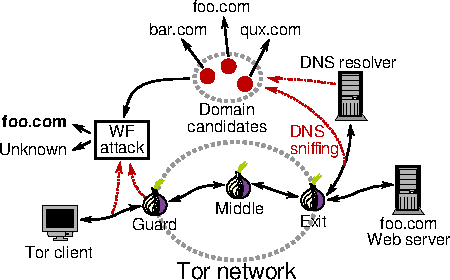
\includegraphics[width=0.8\linewidth]{figures/attack-scenario.pdf}
	\caption{An overview of the \name attack.  An adversary must monitor
		both ingress (encrypted Tor traffic) and egress (DNS request) traffic.
		A AS-level adversary between the
		client and its guard monitors ingress traffic.  The same adversary
		monitors egress traffic between the exit and a DNS server, or the DNS
		server itself.  Both ingress and egress traffic then serve as input to the
		\name attack.}
	\label{fig:attack-scenario}
\end{figure}

\begin{itemize}
    \item \emph{Ingress sniffing:} An attacker must observe traffic that is
		entering the Tor network.  The attacker can operate on the network level,
		as a malicious ISP or an intelligence agency.  In addition, the
		attacker can operate on the relay level by running a malicious Tor guard
		relay.  In both cases, the attacker can only observe encrypted
		data, so packet lengths and
		directions are the main inputs for website fingerprinting~\cite{Panchenko2016a}.
    \item \emph{Egress sniffing:} To observe both ends of the communication, an
		attacker must also observe egress DNS traffic.  We expect the adversary
		either to be on the path between exit relay
		and a DNS server or to run a malicious DNS
		resolver or server.  An attacker may also run an exit relay,
		but in this case conventional end-to-end correlation
		attacks~\cite{Murdoch2007a} are at least as effective as those we
		describe here.
\end{itemize}
We combine a conventional website fingerprinting attack operating on traffic
from ingress sniffing with
DNS traffic observed by egress sniffing, creating \name attacks. Our attacks
correlate the web\emph{sites} observed by the website fingerprinting attack in
ingress traffic with
the web\emph{sites} identified from DNS traffic. Next, we describe how we
simulate the DNS traffic from Tor exits, how we map DNS requests to websites,
and finally present our two \name attacks.

\subsection{Approximating DNS traffic from Tor exits}
\label{sec:attack:sim}

We first investigate the type and volume of DNS traffic that Tor's exit relays
send.  There are no logs of outgoing traffic
from Tor exit relays available to us, and ethical considerations kept us
from trying to collect them (\eg, by operating exit relays and recording
all the outgoing traffic). We therefore opt to approximate the DNS traffic
emerging from Tor exit relays by \first building a model of typical Tor
users' website browsing patterns, \second collecting a minimally invasive
dataset of DNS traffic, and \third accounting for the effects of DNS caching.

\subsubsection{Modeling which sites Tor users visit}
\label{sec:attack:pop}

We first build a model to approximate {which websites} Tor users visit.
As of July 2016, there are about 173 million active
websites~\cite{numberofwebsites}; the Alexa ranking~\cite{alexatop1k}
gives insights into their popularity based on the browsing behavior of
a sample of all Internet users. The distribution of the popularity of
these websites has previously been fit to a power-law distribution based
on the rank of the
website~\cite{Mahanti2013a,Clauset2009a,Ali2007a}.
For the pageview numbers of the Alexa top 10,000 websites, we found a
power-law distribution to be a good fit as neither a log-normal nor a
power-law distribution with exponential cutoff (\ie, a truncated power-law
distribution) offered significantly better fits.
We used the Python {\tt powerlaw} package~\cite{Alstott2014a} for fitting and
picked a power-law distribution with an $\alpha$ parameter of about $1.13$.
When varying the fitting parameter $x_{min}$ that determines beyond which
minimum value the power-law behavior should hold in the provided data, we can
get different $\alpha$ values. We made a conservative choice of picking this
smaller $\alpha$ value as it underestimates the popularity of popular websites
and therefore is worse for the attacker.\footnote{Alexa's page-view numbers
ignore multiple visits by the same user on the same day (see
\url{https://support.alexa.com/hc/en-us/articles/200449744}), so the ranking
might be slightly off when modeling website visit patterns.}
Thus, we use a power-law distribution to model what websites Tor users visit.
This might overestimate the popularity of higher-ranked websites such as
Facebook and YouTube because we believe that Tor users---who tend to be
privacy-conscious---are more likely to seek out alternatives than the typical
Internet user.  We will discuss the implications of our model for browsing
behavior later.

\subsubsection{Modeling how often Tor users visit each site}
\label{sec:load-freq}
% phw's numbers extrapolated
Next, we determine how many websites Tor users visit in a certain time span.
We approximated this number by setting up an exit relay whose exit policy
included only ports 80 and 443, so our relay would only forward web traffic.  We
then used the tool {\tt tshark} to capture the timestamps of DNS requests---but
no DNS responses.  We made sure that our {\tt tshark} filter did not capture
packet payloads or headers, so we were unable to learn what websites Tor users
were visiting.  In addition, we patched {\tt tshark} to log timestamps at a
five-minute granularity. The coarse timing granularity allows us to publish this
dataset with minimal privacy implications; Section~\ref{sec:ethics} discusses
the ethical implications of this experiment in more detail.  We ran the
experiment for approximately two weeks from May 15, 2016 to May 31, 2016, which
allowed us to determine the number of DNS requests for 4,832 five-minute
intervals.  Figure~\ref{fig:dns-reqs} shows this time series.  The
distribution's median is 105, illustrated by the red horizontal line.  The time
series features several spikes; the most significant one counts 1,410 DNS
requests.  We repeated the same experiment with the so-called \emph{reduced exit
policy}\footnote{The reduced exit policy is available online at
\url{https://trac.torproject.org/projects/tor/wiki/doc/ReducedExitPolicy}.}
because it contains several dozen more ports and it is more popular among Tor
relay operators; as of August 2016, it is used by 7.8\% of exit relays by
capacity.  In comparison, the exit policy containing only port 80 and 443 only
accounts for 1.5\%.  The reduced exit policy resulted in a median of 102 DNS
requests per five minutes, so the difference between both policies is only three
DNS requests.

\begin{figure}[t]
	\centering
	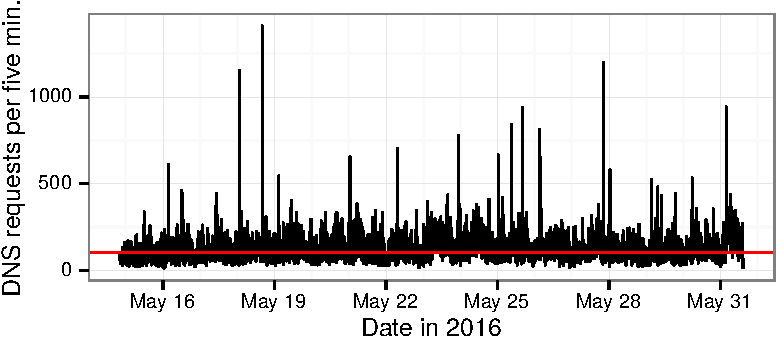
\includegraphics[width=\linewidth]{figures/dns-reqs.pdf}
	\caption{The number of DNS requests per five-minute interval on our
	exit relay.  Using a privacy-preserving measurement method, we only
	determined approximate timestamps and no content.  The red line at $y = 105$
	illustrates the distribution median.}
	\label{fig:dns-reqs}
\end{figure}

We then interpolate these numbers to all Tor exit relays based on their
published bandwidth statistics.  While we measured a median of 105, 
the mean of the distribution was 119.3 per five minutes during a two-week period.
From DNS statistics of the Alexa top one million websites (see
Section~\ref{sec:dns2site}) we know that one website visit causes outgoing DNS requests for 10.3 domains on average
(assuming a power-law distribution of site popularity as described above, and
taking into account Tor's caching of pending DNS requests, ensuring that multiple
requests sent by clients for the same domain name only result in one outgoing request
by the exit).
This means that we had an average of about 23.2 website visits per ten
minutes on our exit relay.  Assuming that the two main factors influencing the
volume of DNS requests are a relay's \emph{bandwidth} and \emph{exit policy},
and having shown that the exit policy does not significantly impact
the number of DNS requests, we can scale this number up to the whole Tor network
using the provided bandwidth of exit relays.  In particular, we use the
self-reported bandwidth information from Tor exit
relays collected in the so-called extra-info descriptors available on
CollecTor~\cite{collector}, and estimate the number of website visits on
each of the about 1,200 exit relays active at that time. The resulting average
total number of websites visited through the Tor network is about 536,000
websites per ten minutes.

Recently, Jansen and Johnson~\cite{Jansen2016a} measured the average
number of active web (port 80 and 443) circuits in Tor to about 700,000 per ten
minutes.\footnote{This number comes from a preprint kindly
shared by the authors and might change in the final version.}
Tor Browser, the Tor Project's fork of Firefox, builds one circuit per
website entered in the URL bar. How long the circuit remains active depends on
Tor Browser settings (primarily {\tt MaxCircuitDirtiness} currently set to ten minutes) and how
long TCP streams in the circuit are active: as long as at least one stream is
active, the circuit remains active. The number of active circuits serves as an
upper bound for the number of websites visited over Tor: visiting different
pages of a website will use the same circuit, and visiting a new website will
construct a new circuit. Users visiting several pages of a website and websites
with long-lived connections, like Twitter and Facebook with continuously
updating feeds,
all lower the number of websites visited in Tor relative to the number of active
circuits. In later sections we revisit the implications of our estimates by
scaling the Tor network to ten-times its estimated size.

\subsubsection{Modeling the effects of DNS caching}
To analyze which DNS requests the adversary can see, we need to
take caching of DNS responses into account. We ignore client-side DNS
caching since it is disabled by default, as described in
Section~\ref{sec:background}.
% From Tobias: I manually could not get Firefox to cache anything,
% not even between pageloads on the same site (went to kau.se, waited 20s,
% then clicked on a link: little tor client-side still got a DNS response
% from the exit for kau.se.)
On the exit relays, which perform DNS resolution on behalf of Tor clients,
caching is relevant because all Tor clients using the same exit relay share its
cache.  An exit relay maintains its own DNS cache%
\footnote{The code is available online at \url{https://gitweb.torproject.org/tor.git/tree/src/or/dns.c?id=tor-0.2.9.1-alpha}.}
(in addition to the cache of its DNS resolver) and enforces a minimum TTL of 60
seconds and a maximum TTL of 30 minutes.%
\footnote{The code is available online at \url{https://gitweb.torproject.org/tor.git/tree/src/or/dns.c?id=tor-0.2.9.1-alpha\#n209}.}
We refer to this as Tor's \emph{TTL clipping}. However, due to a bug in the
source code that we identified,%
\footnote{The bug report is available online at \url{https://bugs.torproject.org/19025}.}
the TTL of all DNS responses is set to 60 seconds.

%\subsubsection{Sliding window approach to compensate for DNS caching}
% we ignore caching by having a window of X minutes
If a Tor client attempts to resolve a domain that the exit relay already has in
its cache, the adversary will be unable to observe this request.  However, the
adversary can record all DNS requests of the exit relay over the past $x$
seconds, where $x$ is the maximum TTL value (\ie, maintain a sliding window of
length $x$), to obtain a lower bound of requested domain names.  If a Tor client
is attempting to resolve a domain name, the request is either cached or not.  If
it is not cached, the adversary will see it as a new, outgoing DNS request from
the exit relay. If it is cached, it must have been resolved by the exit relay in
the last $x$ seconds, and will therefore be in the sliding window.  The sliding
window technique allows the attacker to observe all DNS requests, regardless of
if they are cached or not.

We assume that an adversary applies this sliding window technique and models the
observable DNS data accordingly.  The attacker observes a fraction of Tor's exit
bandwidth for a specific window length, and together with our website visit
frequency estimation, this triggers a number of website visits in our
simulation.  For each visit event, we randomly draw a website using the
power-law website popularity distribution described above and put its DNS
requests into the window. As we will see next, we do not need to simulate or
consider the fact that the observed fraction of Tor exit bandwidth corresponds
to many different exits with individual caches.

\subsection{Inferring website visits from DNS requests}
\label{sec:dns2site}

Given a sliding window of DNS requests, we investigate how this information can
help determine whether a user has visited a website of interest.  In April 2016,
we visited the Alexa top one million websites five times, and collected all DNS
requests that each visit of a website's frontpage generated.  We refer to the
data collected for one visit as a \emph{sample}.  We performed these
measurements in five rounds from a university network, where each round browsed
all one million websites in a random order before visiting the same website
again. We used Tor Browser~5.5.4 and configured it {\em not to browse over Tor}:
Tor Browser ensures that the browser behavior is identical to a Tor Browser user
over Tor. By not using Tor, we can bypass IP blacklists and CAPTCHAs that are
triggered by IP addresses of exit relays~\cite{Khattak2016a}.
Table~\ref{tab:dns-censor} shows the percentage of websites in our dataset that
are hosted by CloudFlare or Akamai.  We might not be able to access these
websites programatically over Tor as they block or filter exit relays, as
identified by Khattak \ea~\cite{Khattak2016a}. We also include Google, which is
prevalent in our dataset and restricts access to Tor users for Google's search.

\begin{table}[t]
	\renewcommand{\tabcaptext}{The percentage of websites on Alexa top-1 million websites using providers
	involved in censoring or restricting access from
        Tor~\protect\cite{Khattak2016a}.}
      \topcap{\tabcaptext}
	\centering
	\begin{tabular}{l r}
	\toprule
	\textbf{Description} & \textbf{Percentage} \\
	\midrule
	Website behind CloudFlare IP & 6.44 \\
	Domain on website uses CloudFlare & 25.81 \\
	Domain on website uses Akamai & 33.86 \\
	Domain on website uses Google & 77.43 \\
	\bottomrule
	\end{tabular}
        \bottomcap{\tabcaptext}
	\label{tab:dns-censor}
\end{table}

We collected 2,540,941 unique domain names from a total of 60,828,453 DNS
requests. The dataset contains 2,260,534 domains that are unique to a particular
website, \ie, are not embedded on any other top million site; we call these
domains {\em unique domains}. Unique domains are particularly interesting
because they reveal to the adversary what sites among the top million the user
has visited.  This is not possible for domains such as {\tt youtube.com}, simply
because many websites embed YouTube videos.  Figure~\ref{fig:unique-domains}
shows the fraction of sites with unique domains for websites up to Alexa's top
one million.  We grouped all domains into 1,000 non-overlapping bins of size
1,000.  For 96.8\% of all sites on the Alexa top one million there exists at
least one unique domain.  Interestingly, more popular websites are less likely
to have a unique domain associated with them: only 77\% of the first bin---the
most popular 1,000 domains---contain at least one unique domain, significantly
less than the rest of the data.

Table~\ref{tab:dns-domains} shows summary statistics for the number of domains
per website. At least half of the sites have ten domains per website, two of
them are unique, suggesting that an adversary can identify many website visits
by observing a single unique DNS request.

\begin{figure}[t]
	\centering
	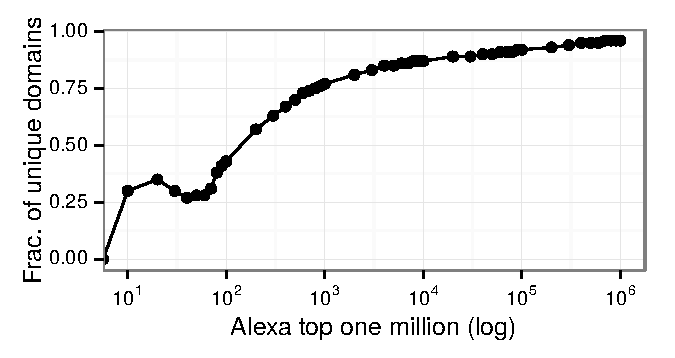
\includegraphics[width=0.75\linewidth]{figures/dns-unique-domains.pdf}
	\caption{The fraction of websites in Alexa's top one million that have at
	least one unique domain.  We grouped all domains into 1,000 non-overlapping
	bins of size 1,000.  The vast majority of sites (96.8\%) have unique
	domains.}
	\label{fig:unique-domains}
\end{figure}

\begin{table}[t]
	\renewcommand{\tabcaptext}{Summary statistics for the number of domains per
	website in the Alexa top 1 million. More than half of the sites embed two
	domains that are unique to that site.}
	\topcap{\tabcaptext}
	\centering
	\begin{tabular}{l r r r r}
	\toprule
	\textbf{Domains} & \textbf{Median} & \textbf{Mean $\pm$ Stddev} & \textbf{Min.} & \textbf{Max.} \\
	\midrule
	Per site & 10 & $12.2\pm11.2$ & 1 & 397 \\
	Unique per site & 2 & $2.3\pm\phantom{0}1.8$ & 0 & 363 \\
	\bottomrule
	\end{tabular}
        \bottomcap{\tabcaptext}
	\label{tab:dns-domains}
\end{table}



To evaluate the feasibility of mapping DNS requests to websites, we
construct a na\"{\i}ve website classifier that maps the unique domains
in a set of DNS requests to the corresponding website that contains a
matching set of domains.  With five-fold cross-validation on our Alexa
top one million dataset (with five samples per site),
we consider a closed world and an open world.
In the closed world, the attacker can use samples
from all sites in training; in the open world, some sites
are unmonitored and therefore unknown (as per the fold).  The
closed-world evaluation yields 0.955 recall.  In the open-world
evaluation, we monitor the Alexa top 500,000 with five samples each and
consider 433,000 unmonitored sites.  The number of unmonitored sites is
determined by our power-law
distribution to represent a realistic base rate (for the entire Tor network)
for evaluating our classifier: on average, for sites on Alexa top 500,000
to be visited 2.5 million times there will be about 433,000 visits to sites
outside of Alexa top 500,000.  Our classifier does not take into account the
popularity of websites.
The open-world evaluation yields a
recall of 0.947 for a precision of 0.984.  By accounting for the order
of requests, per-exit partitioning of DNS requests, TTLs, and website
popularity, we expect that classifying website visits from DNS requests
might be made even more accurate.
Further, a closed world is a realistic setting:
determining the DNS requests made by all 173 million active websites on the
Internet is practical, even with modest resources.
We use the conservative open world results when simulating the Tor network and
the attacker's success in mapping DNS requests to websites.
We conclude from our results that observing DNS requests coming out of Tor is
almost as effective at identifying websites as observing the web traffic
itself.

\subsection{Classifiers for \name attacks}

We use Wa-kNN from Wang \ea~\cite{Wang2014a} (described in
Section~\ref{sec:background}) and a list of sites derived from
observing DNS requests to implement two \name attacks:

\begin{description}
	\item[\texttt{ctw}] We ``close the world''
	on a Wa-kNN classifier that we modified to consider only the distance to
	observed sites when calculating the $k$-nearest neighbors.
	The classifier still considers the distance to all unmonitored sites.
	\item[\texttt{hp}] When Wa-kNN classifies a trace as a monitored site, confirm
	that we observed the same site in the DNS data (ensuring {\em high
	precision}). If not, make the final classification unmonitored.
\end{description}
\noindent
These approaches apply to any website fingerprinting attack. The
\texttt{ctw} attack increases the effectiveness of conventional website
fingerprinting attacks by making them more akin to a closed-world setting,
where websites have known fingerprints and often the world is of limited size.
Conceptually, the attack could also include
a custom weight-learning run---training only on observed sites---but our initial
results noted little to no gain, despite significant increases in
testing time.
We expect that this is due to the fact that some features of traffic traces are
more useful than others, regardless of the training data~\cite{Hayes2016a}.
The \texttt{hp} attack only produces a positive classification if both ingress
and egress traffic are consistent, resulting in a simple but effective
classifier.
